
% \global\long\def\figHeight{3.3cm}
\begin{figure}[t]
    % \includegraphics[width=\textwidth]{inkscape/eyecatch.png}
    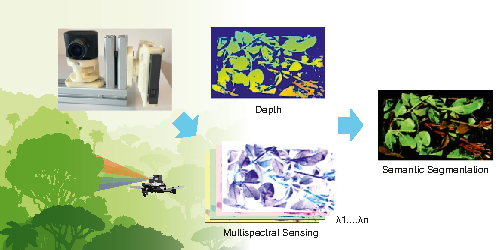
\includegraphics[width=0.5\textwidth]{chapters/papers/ED/resources/figures/figure_1_inspiration.pdf}
    \caption{Event Spectroscopy motivation, an all-in-one, ambient-light independent solution for depth sensing, RGB image reconstruction and multispectral sensing. Usable for instance, for an uncrewed aerial vehicle (UAV) navigating in forest environments.  (a) Our setup consisting of an event camera and a projector as an illumination source 
    (b) Depth of scene acquired using structured light (c) RGB image reconstructed from events, (d) Spectral image reconstructed using events (e) Material segmentation of fern leaves using spectral and depth data.} 
    \label{fig:eye} 
\end{figure}
